\documentclass{article}
\usepackage{tikz}
\usetikzlibrary{patterns}
\usetikzlibrary{shapes.geometric}
\title{CSE 300 Practice on tikZ}
\author{1605042}
\date{\today}
\tikzstyle{myBox} = [trapezium,trapezium left angle=60,trapezium right angle=120]
\begin{document}
	\maketitle
	
\section{practice on ticz}
\begin{tikzpicture}
	\draw (0,0)--(2,3)--(4,0);
	\draw (0,0)..controls(2,3)..(4,0);
\end{tikzpicture}
\vskip25pt

\begin{tikzpicture}
\draw (1,0) -- (0,0) -- (0,1) (0,0) -- (1,1);
\end{tikzpicture}

\vskip25pt

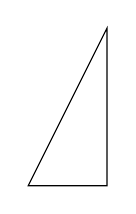
\begin{tikzpicture}
\draw (3,0)--(4,0)--(4,2)--cycle;
\end{tikzpicture}

\vskip25pt

\begin{tikzpicture}
\draw[color=red,scale=1.5] (0,0) rectangle (2,3);
\end{tikzpicture}

\vskip25pt

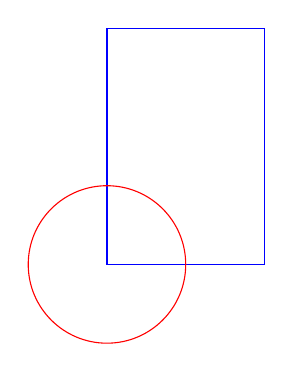
\begin{tikzpicture}
\draw[color=blue] (0,0) rectangle (2,3);
\draw[color=red] (0,0) circle [radius=1];
\end{tikzpicture}

\vskip25pt

\begin{tikzpicture}
\draw[color=red] (0,0) circle [radius=2];
\end{tikzpicture}

\vskip25pt

\begin{tikzpicture}
\draw (0,0) arc[start angle=30, end angle=90, radius=1cm];
\draw (3,0) arc(30:90:3cm);
\end{tikzpicture}

\vskip25pt

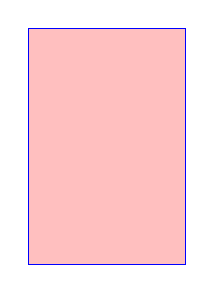
\begin{tikzpicture}
\filldraw[draw=blue,fill=pink] (0,0) rectangle (2,3);
\end{tikzpicture}

\vskip25pt

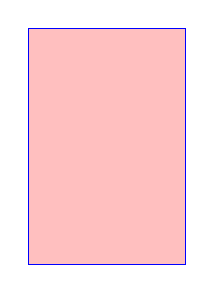
\begin{tikzpicture}
\filldraw[draw=blue,fill=pink] (0,0) rectangle (2,3);
\end{tikzpicture}

\vskip25pt

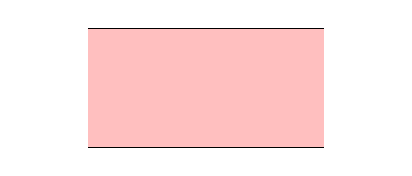
\begin{tikzpicture}
	\draw[double,double distance=15mm, double=pink ] (0,0)--(3,0);
\end{tikzpicture}
\vskip25pt
\begin{tikzpicture}
\draw[<-> ] (0,0)--(3,0);
\end{tikzpicture}
\vskip25pt
\begin{tikzpicture}
\draw[<-> ] (0,0)-|(3,3);
\end{tikzpicture}
\vskip25pt
\begin{tikzpicture}
\draw[<-> ] (0,0)|-(3,3);
\end{tikzpicture}
\vskip25pt
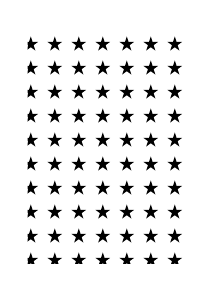
\begin{tikzpicture}
\pattern[pattern=fivepointed stars] (0,0) rectangle (2,3);
\end{tikzpicture}
\vskip25pt
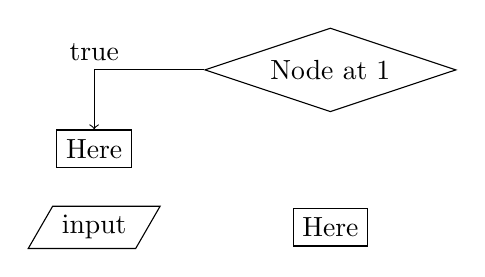
\begin{tikzpicture}
\node[draw,diamond,aspect=3] (n1) at (3,0){Node at 1};
\node[draw,below of=n1,yshift=-1cm] (n2) {Here};
\node[draw,left of=n1,yshift=-1cm,xshift=-2cm] (n3) {Here};
\node[draw,myBox,below of=n3](n4) {input};
\draw[->] (n1.west) -| node [above]{true}(n3.north);
\end{tikzpicture}



\end{document}